% Created 2017-09-22 sex 09:13
% Intended LaTeX compiler: pdflatex
\documentclass{report}
               \pagestyle{fancy}
\usepackage[latin1]{inputenc}
\usepackage[T1]{fontenc}
\usepackage{graphicx}
\usepackage{grffile}
\usepackage{longtable}
\usepackage{wrapfig}
\usepackage{rotating}
\usepackage[normalem]{ulem}
\usepackage{amsmath}
\usepackage{textcomp}
\usepackage{amssymb}
\usepackage{capt-of}
\usepackage{hyperref}
\usepackage{paralist}
\usepackage{tcolorbox}
\usepackage[table]{xcolor}
\usepackage{lipsum}
\usepackage{caption}
\usepackage{tabu}
\usepackage[subpreambles=true]{standalone}
\usepackage{import}
\usepackage{setspace}
\usepackage{graphics}
\usepackage[linktocpage=true]{hyperref}
\usepackage{tocloft}
\usepackage{minitoc}
\usepackage[portuguese, english]{babel}
\usepackage{subfig}
\usepackage[utf8]{inputenc}
\date{}
\title{}
\hypersetup{
 pdfauthor={},
 pdftitle={},
 pdfkeywords={},
 pdfsubject={},
 pdfcreator={Emacs 25.2.1 (Org mode 9.0.9)}, 
 pdflang={English}}
\begin{document}

\thispagestyle{firstpagestyle}

\import{latex/}{side_info}

\pagestyle{plain}
  \begin{tcolorbox}[colbak=red!5!white, colframe=red!0!white]
  \large{
  \textbf{Highlights}
  \vspace{0.1cm}
  \it
    \import{latex/}{highlights}
  }
  \end{tcolorbox}
  \vspace{-0.4cm}

\setlength{\parindent}{0cm}
\setlength{\parskip}{0.1cm}

\textbf{Global Markets.} European equities are up, and the S\&P future is
edging down by 0.1\%. The Mexican peso is noticeably up by 0.4\% against
the USD, and the yield of the 10 years Treasury is sliding to
2.25\%. Commodities: oil is marginally down 0.1\% to USD50.5, steel is
down 2.2\% and soy prices is climbing by about 0.9\%.

\textbf{Local News}. \textbf{Politics.} The second charge against Temer has finally
been sent to the Lower House. Against this background, the O Estadao
reiterates the Speaker of House discontentment with the PMDB, which
has interfered on his party's election strategy, and may impair the
processing of the charge in the House. At the other extreme, the media
outlet Broadcast informs Mr. Rogrigo Maia is, nonetheless, resolved to
get done and over with it in a expedience manner.

In addition, as we have noticed in our visit to Brasilia this week,
the O Valor noticed that PSDB looks more tamed now and,
partially sponsored by the Governor of Sao Paulo, may deliver more
votes to Temer in this time around. As expected, however, the Estadao
reports that PP, PR and PSD are again complaining about their
relationship with the government, and taking up the opportunity to
raise their stakes for more room in the government.

The presidential election race also occupies some importance. As
matter of fact, Mr. Alckmin move to sooth the government would be indeed a
step to neutralize Mr. Doria's advancements within the PMDB. In the
meantime, the latter and Mr. Rodrigo Maia seem to be in courtship
mode, after having dinner last night. Finally, according to the O
Valor, the Mr. Henrique Meirelles' name would be gathering strength
and should the economy take off for good, his candidacy could take off
for real.

\textbf{On the fiscal front}, the \textbf{Refis} comes back to the fore yet again and,
as we informed yesterday, the speculation the government may not renew
its provisional measure continues, which is raising anxieties in the
Congress, since it would like to see the approval of softer
version. Meanwhile, the \textbf{Cemig's} soup opera leaves on. Although its
auction is scheduled to next week, the companies is trying to postpone
in order to strike a last minute deal with the government.

Finally, \textbf{on the economic camp}, newspapers comes filled with optimism
on the back of a discussion over yesterday's \textbf{Quarterly Inflation}
report by the Central Bank. In a nutshell, annalists and commentators
alike are raising the bets of low interest rates for longer amid
higher GDP growth.

\textbf{Agenda - Highlights}: \uline{Brazil}: Consumer confidence - FGV, September
and Industrial Confidence - CNI, September. \uline{US}: Markit US PMI,
September.

\rowcolors{2}{grey!15}{white}
\vspace{-0.5cm}

\begin{center}
\begin{tabular}{rlllll}
\textbf{Time} & \textbf{Country} & \textbf{Indicator} & \textbf{Period} & \textbf{Forecast} & \textbf{Impact}\\
\hline
08:00:00 & BZ & Consumer Confidence @ 82,3 & Sep & - & low\\
10:45:00 & US & Markit Manufac. & Sep P & 53 & Medium\\
10:45:00 & US & Markit Services & Sep P & 55,7 & Medium\\
11:00:00 & BZ & CNI Business confidence & Sep & - & Low\\
\end{tabular}
\end{center}

\textbf{Bottom Line}. Global markets looked mixed, while local news comes
plenty optimism, which may set a positive mode for local markets.

\newpage

\section{Brazilian Bonds}
\label{sec:org5e5b2cb}


\begin{center}
\textbf{NTNF} \\
\vspace{0.1cm}
\import{latex/}{NTN-F}
\end{center}
\vspace{0.5cm}

\begin{center}
\textbf{LTN} \\
 \vspace{0.1cm}
\import{latex/}{LTN}
\vspace{0.5cm}
\end{center}

\begin{center}
   \textbf{NTN-B} \\
\vspace{0.1cm}
       \import{latex/}{NTN-B}
       \vspace{0.1cm}
     \end{center}
     \newpage



\begin{center}
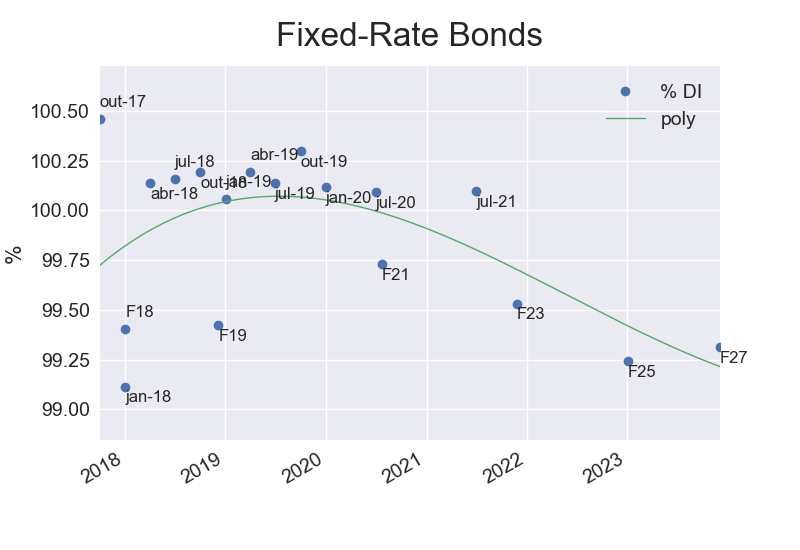
\includegraphics[width=16.0cm]{charts/fixed.png}
\end{center}

\begin{center}
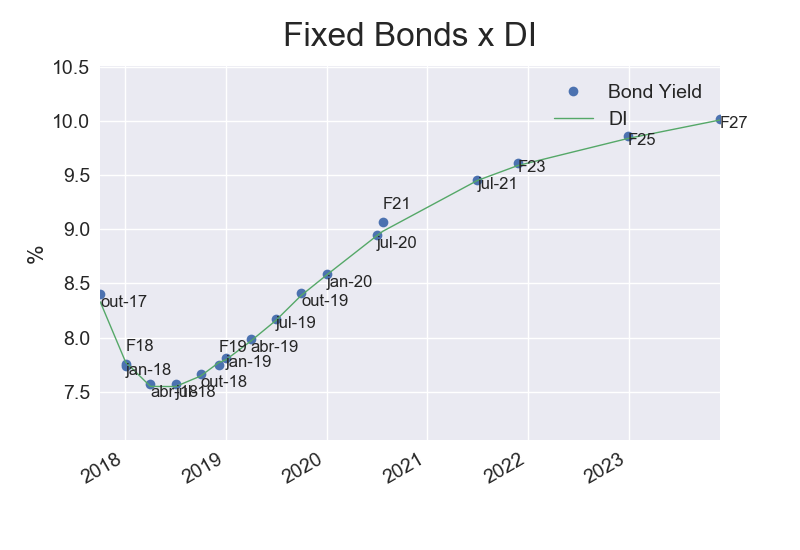
\includegraphics[width=16.0cm]{charts/fixed_di.png}
\end{center}

\begin{center}
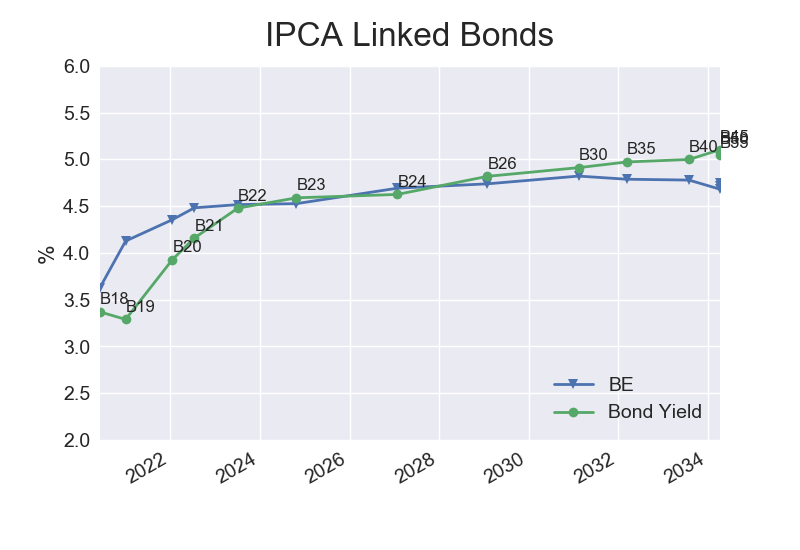
\includegraphics[width=16.0cm]{charts/ntnb.png}
\end{center}


\section{DI - Open Interest}
\label{sec:org71c6115}

  \begin{center}
    \import{latex/}{OpenInterest}
  \end{center}
\newpage

\vspace{3.0cm}
  \begin{center}
    \import{latex/}{DIContracts}
  \end{center}
\newpage


\section{DI - DV01 Table}
\label{sec:orgc699158}

  \begin{center}
    \import{latex/}{DIs}
  \end{center}
\newpage


\section{NTNB FRAs}
\label{sec:org89b3a29}


\begin{center}
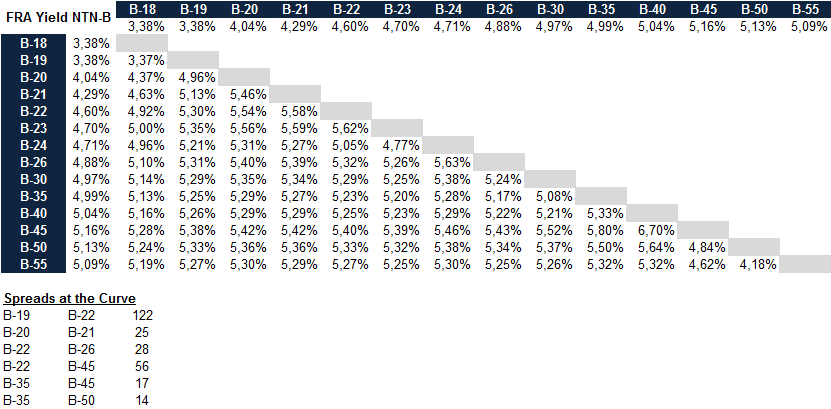
\includegraphics[angle=90,width=10.5cm]{images/FRA_NTNB.png}
\end{center}

\newpage


\section{DI FRAs}
\label{sec:orgf3cc546}
\begin{center}
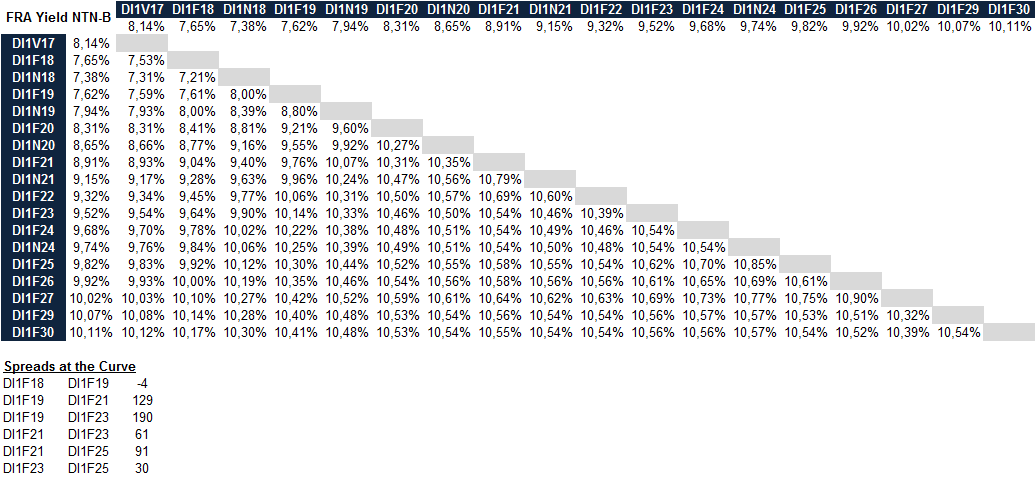
\includegraphics[angle=90,width=10.5cm]{images/FRA_DI.png}
\end{center}

\newpage


\section{Disclaimer}
\label{sec:org7cac1ed}
\smallsize
\begin{quote}
This report has been produced by Guide Investimentos S.A Corretora de
Valores solely for its recipients and should not be distributed
without previous consent from Guide Investimentos S.A.  Although this
report is based upon the most reliable public information, Guide
Investimentos makes no warranties of the reliability of such
information. This document is for informational purposes only and does
not constitute any tender to sell or buy financial
instruments. Information discussed herein is not suitable for all
investors and it does not aim at providing any trading strategy for
individual goals. Investors should have experience and knowledge of
the risks in FX/Fixed Income markets. Guide Investimentos S.A
Corretora de Valores has no obligation to update, revise or modify any
information contained herein. Guide Investimentos and its analysts
shall not be held responsible for any accidental incorrect
information, nor for investment decisions taken based upon the
information contained herein. Additional information discussed on this
report is available upon request.  Analysts each certify that the
views expressed in this report represent only personal views produced
independently, including with respect Guide Investimentos S.A
Corretora de Valores. This report should not be considered as research
report ("relat�rio de an�lise") for the purposes of the article 1 of
CVM Instruction NR 483. Opinions, estimates and projections contained
herein express the current judgment of the analysts build on the date
this report was released and therefore can be changed without
notice. Analysts do not accept any liability that incorrect use of
this report could cause, including financial losses. Upon accepting
this document, one should agree with all the above-mentioned
limitations
\end{quote}
\end{document}
